% This is samplepaper.tex, a sample chapter demonstrating the
% LLNCS macro package for Springer Computer Science proceedings;
% Version 2.20 of 2017/10/04
%
\documentclass[runningheads]{article}
%
\usepackage{graphicx}
\usepackage[left=3cm, right=3cm]{geometry}
% Used for displaying a sample figure. If possible, figure files should
% be included in EPS format.
%
% If you use the hyperref package, please uncomment the following line
% to display URLs in blue roman font according to Springer's eBook style:
% \renewcommand\UrlFont{\color{blue}\rmfamily}

\begin{document}
%
\title{A TAS on : Navigating the Bumpy Road from Engineer to Manager}
%
%\titlerunning{Abbreviated paper title}
% If the paper title is too long for the running head, you can set
% an abbreviated paper title here
%
\author{Author: Dhyey Doshi (40244534)}
%
% \authorrunning{F. Author et al.}
% First names are abbreviated in the running head.
% If there are more than two authors, 'et al.' is used.
%
% \institute{Concordia University
% \email{lncs@springer.com}\\
% \url{http://www.springer.com/gp/computer-science/lncs} \and
% ABC Institute, Rupert-Karls-University Heidelberg, Heidelberg, Germany\\
% \email{\{abc,lncs\}@uni-heidelberg.de}

%
\maketitle              % typeset the header of the contribution
%
\begin{abstract}
The transition from an engineering role to a managerial position is often challenging, marked by a shift from objective, technical tasks to subjective, people-oriented responsibilities. This journey is frequently fraught with uncertainty, as the metrics for success become less tangible, and the feedback loop elongates. Many first-time engineering managers grapple with feelings of un-productivity and anxiety, leading some to retreat to hands-on technical work. This article explores ways to smooth the bumpy road of transitioning from an engineer to a manager, emphasizing a mindset shift and the importance of recognizing the impact of managerial actions. The key elements discussed include self-reflection through daily impact logs, seeking internal peer support, and engaging external coaching to illuminate the rewards and impact of the managerial path. By addressing these aspects, the article aims to provide guidance for a smoother and more fulfilling transition into engineering management.
\end{abstract}
%
%
%
\section{Introduction}
\subsection{Motivation}
The motivation behind this topic lies in the common difficulty experienced by engineers transitioning into managerial roles, often resulting in a lack of support and understanding of the impact of managerial actions.
The overall goal is to enhance the experience of individuals entering managerial roles by addressing difficulties, offering strategies for a smoother transition, and emphasizing the importance of mindset shifts and establishing a support network.

\subsection{Problem statement}
The issue is determining the challenges, responsibilities, and abilities required for a smooth transition. There is a need to investigate the reasons why engineers may choose to go into management positions, such as the potential to have a larger effect, acquire leadership abilities, and take on new challenges. Looking into the technical and soft skills, networking, education, and management experience that are required for success in a management post is essential. Moreover, engineers need advice on how to prepare for the shift, what to expect in a managerial role, and the potential hazards and trade-offs associated with making this transition.

\subsection{Objectives}
Investigating how to navigate the road from engineer to manager can help individuals, organizations, and the engineering community.
\begin{itemize}
    \item Individuals can get advice on the skills and information needed for a successful transition, as well as the potential challenges and rewards.
    \item It can assist organisations realise the importance of engineering management and the influence it can have on their success.
    \item It can also aid the engineering community by providing insights into the changing nature of engineering roles and the abilities required to flourish in management positions. 
\end{itemize}
Overall, this research can help engineers' professional development, organisational success, and the advancement of the engineering sector as a whole.

\section{Background}
\subsection{The challenges of transitioning from an engineer to an engineering manager}

Transitioning from an engineer to an engineering manager presents a range of challenges. These encompass the acquisition of novel skills such as leadership, communication, and conflict resolution, along with an understanding of the new duties inherent in the managerial role. Entrusting tasks to others and relying on them to align with your vision poses a substantial challenge, especially for individuals inclined towards perfectionism. Effectively managing time is a nuanced aspect, devoid of a universal solution. Moreover, the shift from an individual contributor to overseeing a team necessitates a considerable adjustment in mindset and priorities.
\subsubsection{Some more challenges include}
\begin{itemize}
    \item Mindset: Engineers are used to solving problems hands-on. Whereas a manager has to look into the consequences and and look for a more strategic and company-minded approach
    \item People management: Managing people involves understanding team dynamics, resolving conflicts, and fostering collaboration.
    \item Communication Skills: As a manager, clear and effective communication becomes paramount. There is also a need to motivate the people using powerful words.
    \item Time Management: It becomes crucial in order to address both immediate issues and long-term goals.
    \item Adapting to Change: The technology landscape and business environments are constantly evolving. Managers must adapt to change and stay updated on industry trends.
    \item Feedback: Offering constructive feedback, both positive and negative, is an essential part of managing a team. Whereas, a manager should also be ready to get some feedback 
\end{itemize}

While the role of an engineering manager is demanding, it offers personal and professional satisfaction, providing an avenue to make a substantial impact on the company, collaborate with individuals, and nurture the next generation of leaders.

\subsection{Common patterns of failure}

\subsubsection{Failure to Adapt Attitudes to Managerial Role: \\}
Managers who do not adjust their attitudes regarding "people versus things" and "soft versus hard skills" for their new role may face failure. There have been cases of managers not trusting others and involving themselves into technical tasks rather than focusing on the managerial responsibilities.

\subsubsection{Directors Reinforcing Technical Focus: \\}
If the Board of Directors evaluates the manager based on technical troubleshooting rather than management performance, it reinforces the above mentioned pattern of failure.

\subsubsection{Perfectionism Leading to Bottleneck: \\}
The engineer's orientation towards perfection and professional excellence may hinder the flow of work. The manager may be overly critical of subordinates' work, rechecking or even reworking it to meet their own standards - leading to overall failure.

\subsection{Notable examples of transitions from engineer to manager}

\begin{enumerate}
    \item Satya Nadella:

    Background: Satya Nadella started at Microsoft as an engineer. He later transitioned to leadership roles, eventually becoming the CEO of Microsoft in 2014.

    Key Takeaway: Nadella's ability to lead and transform Microsoft showcases the potential for engineers to rise to the highest levels of leadership.

    \item Sundar Pichai:
    
    Background: Sundar Pichai started as an engineer at Applied Materials and later worked at McKinsey and Company. He joined Google in 2004 and gradually rose through the ranks to become the CEO of Google and Alphabet.
    
    Key Takeaway: Pichai's career progression illustrates how a combination of technical expertise and leadership skills can lead to the top executive role in a major tech company.

    \item Ginni Rometty:

    Background: Ginni Rometty, the former Chairman, President, and CEO of IBM, started as a systems engineer. She progressed through various roles at IBM, leading global sales and marketing before becoming the CEO.
    
    Key Takeaway: Rometty's story emphasizes the importance of diverse experiences within the same company and the ability to take on different challenges to reach top leadership roles.

\end{enumerate}

\section{METHODS \& METHODOLOGY}

\subsection{Solutions suggested by the author "Jean Hsu"}
Encouraging a fundamental mindset shift is vital and for that, there are three solutions suggested:
\begin{enumerate}
    \item Keeping a Log: 

    Maintaining a log proves advantageous for engineering managers in various aspects. It establishes accountability within the management team, as the manager can define specific criteria for the information they require, ensuring the completion of essential tasks. This approach also grants access to vital metrics and data, eliminating the need for constant follow-ups with the team. Furthermore, it facilitates enhanced communication by enabling the sharing of crucial data and information among team members. \\

    \item Looking for Peer Support: 

    The journey of transitioning from an engineer to a manager is complex, and having a network of reliable peers can greatly simplify this process. Colleagues within the organization can serve as a valuable resource, acting as a sounding board and offering insights into the dynamics of the company. They provide guidance on the challenges inherent in managerial roles, drawing from their own experiences to shed light on the nuances of the position. This includes practical advice on team leadership, strategic decision-making, and effective communication. \\

    \item Working with a coach 

    Engaging with a coach significantly eases the shift from an engineer to a manager by offering invaluable support, guidance, and a fresh perspective. A coach becomes a reliable partner, shedding light on the individual's strengths and areas for improvement, fostering the crucial self-awareness needed for personal growth. Through providing clarity and aiding in making well-informed career decisions, a coach empowers first-time managers to navigate their managerial roles with assurance. Going beyond personal development, coaches play a pivotal role in refining interpersonal skills, imparting effective delegation techniques, and instilling time management proficiency. \\
    
\end{enumerate}


\subsection{Some other solutions: }

\textbf{Develop Leadership Skills: } such as communication and conflict resolution. \\
\textbf{People Management: } Recognize that managing people is not the same as managing tasks. Put your attention towards developing bonds with those around you. \\
\textbf{Time Management: } A manager requires to take quick decisions. Set priorities and manage time effectively. It is best to delegate efficiently to keep the attention on high-priority projects. \\
\textbf{Decision Making: } Managers often need to make tough decisions. Developing the ability to make informed and timely decisions, considering both short-term and long-term effects is crucial. \\
\textbf{Continuous Learning: } A manager must maintain current knowledge of management strategies, industry developments, and leadership practises. To improve managerial skills, one can attend workshops, seminars, or pursue further education. \\


\section{Plausible Arguments and Limitations}

While the suggested solutions by the author Jean Hsu can be beneficial for many individuals, but according to me it is important to consider potential counterarguments:

\begin{enumerate}
    \item Limitations for keeping a log:

    Maintaining a daily log can be time-consuming, and some people may find it difficult to consistently reflect on their activities. This may be especially true for those who work in fast-paced environments with numerous and urgent daily tasks. \\
    Individuals may struggle to accurately gauge the downstream effects of their work because the impact of actions can be subjective. This subjectivity has the potential to undermine the efficacy of this reflective exercise. \\

    \item Limitations for finding peer support:

    Relying solely on peer support may limit exposure to different points of view. A group of peers may have similar experiences or biases, making it possible to miss out on alternative perspectives that could provide valuable insights. Additionally, Individuals may be hesitant to openly discuss challenges and concerns with peers due to concerns about breaches in confidentiality or potential negative repercussions. \\

    \item Limitations for working with a coach:

    Not everyone or every company has the financial means to hire a coach, and access to coaching services may be limited. This may result in disparities in the assistance available to engineers seeking guidance in their transition to management. Furthermore, the effectiveness of coaching can differ depending on the coach's experience and approach.  \\
    
\end{enumerate}

\section{CONCLUSIONS AND FUTURE WORKS}

\subsection{Conclusion}

In conclusion, an engineering manager's job is to efficiently complete tasks with the assistance of others. For this, Jean Hsu's article underscores the need for a fundamental mindset shift, impact recognition, and a strong support network to navigate the challenging transition from engineer to manager successfully. 

Individuals who adopted the daily impact logs reported a heightened awareness of the broader consequences of their managerial actions, leading to a more positive self-perception and increased job satisfaction. The establishment of internal peer support networks has proven beneficial, fostering a culture of collaboration and shared learning. External coaching has provided individuals with personalized guidance, resulting in improved decision-making and a clearer understanding of the rewards and impact of the managerial path.

\subsection{Real World Applications}

\begin{itemize}
    \item Communication Skills. Application: Communicating project updates and goals with team members, presenting ideas to stakeholders, and facilitating effective team meetings.

    \item Time Management. Application: Juggling multiple projects, meetings, and deadlines, ensuring that tasks are prioritized effectively to meet project milestones and deliverables.

    \item Strategic Thinking. Application: Aligning team goals with overall business objectives, anticipating industry trends, and adapting strategies to meet changing market conditions.

    \item Delegation. Applications: Assigning tasks based on team members' strengths, empowering them to take ownership of their responsibilities, and fostering a sense of accountability.

    \item Networking and Support. Application: Building relationships with colleagues, attending industry events, and seeking advice from mentors or peers to enhance professional growth.
\end{itemize}

\section{Future Works}

\begin{itemize}
    \item AI and Automation Integration: The incorporation of AI and automation technologies facilitates the shift of engineers into managerial positions, as it optimizes engineering processes, improves project management, and promotes innovation and collaboration. Through the automation of routine tasks and the simplification of intricate procedures, engineers can dedicate more attention to creative problem-solving and higher-level decision-making.

    \item Agile and Adaptive Leadership: Agile and adaptive leadership underscores the importance of flexibility, learning, and collaboration. Leaders following an agile approach can modify their strategies, processes, and behaviors in response to feedback and evolving circumstances. This empowerment enables their teams to experiment, innovate, and provide value to customers.

    \item Neuroleadership: It is a discipline delving into the neural foundations of leadership and management methods, offers valuable insights for engineers making the shift to managerial positions. By understanding how brain works, it provides understanding in areas such as decision-making, emotional regulation, collaboration, influence, and mindfulness.
    
\end{itemize}



% \begin{figure}
% 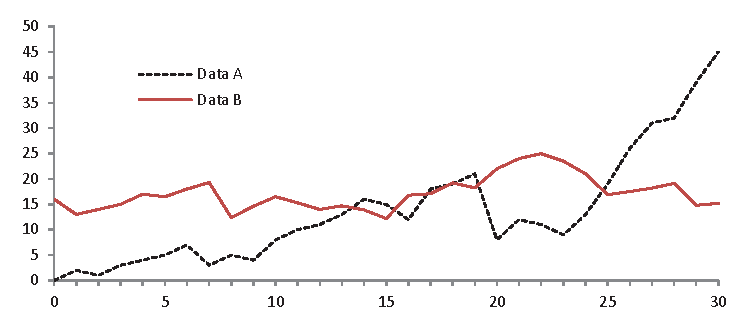
\includegraphics[width=\textwidth]{fig1.eps}
% \caption{A figure caption is always placed below the illustration.
% Please note that short captions are centered, while long ones are
% justified by the macro package automatically.} \label{fig1}
% \end{figure}

%
% ---- Bibliography ----
%
% BibTeX users should specify bibliography style 'splncs04'.
% References will then be sorted and formatted in the correct style.
%
% \bibliographystyle{splncs04}
% \bibliography{mybibliography}
%
\begin{thebibliography}{8}
\bibitem{1}
Utilities One. (2023). Title: The Road to Engineering Management: Essential Steps for Advancement in Your Career
\bibitem{2}
VIKTOR STOJANOV. (2023). Title: Challenges when switching from Engineer into Management. Website title: Babbel Magazine
\bibitem{3}
Koplow, R. A. (1967). From engineer to manager—And back again. IEEE Transactions on Engineering Management, (2), 88-92.
\bibitem{4}
David Scott Peters. (2022). Title: Top 3 Reasons to Use a Manager Log
\bibitem{5}
Jean Hsu. (2017). Title: Navigating the bumpy road from engineer to engineering manager
\bibitem{6}
Amtec Team. (2023). Title: The Impact of AI and Automation on the Engineering Workforce
\bibitem{7}
McPherson, B. (2016). Agile, adaptive leaders. Human Resource Management International Digest, 24(2), 1-3.
\bibitem{8}
Nesta. (2019). Title: Neuroleadership and management
\bibitem{9}
Boyd, E. L. (1978). The transition of an engineer to an engineering manager: the people problem.
\bibitem{10}
Mhlongo, S. (2017). The transition from engineer to manager: implications for the effectiveness of the engineer-in-training programme at Tongaat Hulett–Sugar (Doctoral dissertation).
\bibitem{11}
Author, F.: Article title.
\end{thebibliography}

\section{Acknowledgements}
\begin{itemize}
    \item https://www.perplexity.ai/ (Perplexity) - The capabilities of Perplexity played a crucial role in expanding the scope of research and enhancing the overall coherence, grammar and correctness of the report.
\end{itemize}

\end{document}
